\colorlet{punct}{red!60!black}
\definecolor{background}{HTML}{EEEEEE}
\definecolor{delim}{RGB}{20,105,176}
\colorlet{numb}{magenta!60!black}

\lstdefinelanguage{json}{
basicstyle=\normalfont\ttfamily,
showstringspaces=false,
breaklines=true,
frame=lines,
backgroundcolor=\color{background},
literate=
{:}{{{\color{punct}{:}}}}{1}
{,}{{{\color{punct}{,}}}}{1}
{\{}{{{\color{delim}{\{}}}}{1}
{\}}{{{\color{delim}{\}}}}}{1}
{[}{{{\color{delim}{[}}}}{1}
{]}{{{\color{delim}{]}}}}{1},
}



In de klasse Screen , is er een functie die van een canvas in de grootte van de originele foto van de opstelling het gedeelte van zijn eigen scherm kan knippen en transformeren met een perspectief transformatie, zie figuur \ref{remapDiagram}.

Er is dus een canvas met de juiste grootte van het scherm waarop een gekozen foto op geplaatst kan worden. Deze foto kan verschoven worden met de muis. Eens de foto op de gewenste plaats staat wordt elke scherm er uitgeknipt, getransformeerd.

Eens de transformatie klaar is wordt de foto naar een base64 string geconverteerd en verzonden in json formaat via de socket met endpoint 'screenCommand', zie figuur \ref{json}

\vspace{30px}

\begin{figure}
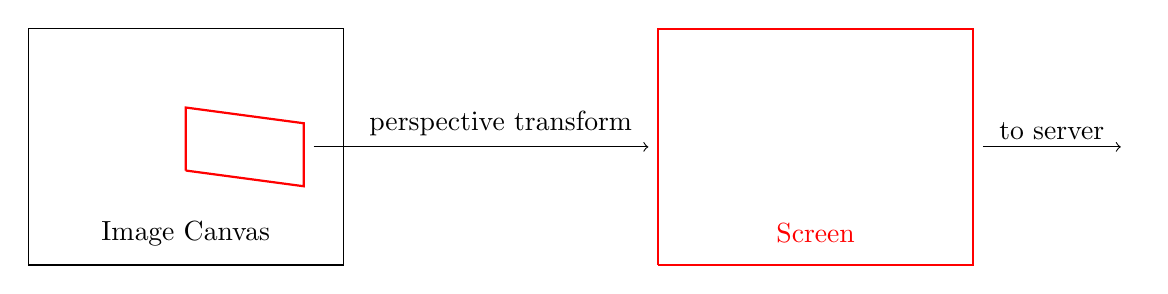
\begin{tikzpicture}
\node (A) at (3.5, 1.5){};
\node (B) at (8,1.5){};
\node (C) at (6,1.8){perspective transform};
\node[red] (D) at (10,0.4){Screen};
\node (E) at (2,0.4){Image Canvas};
\node (F) at (12,1.5){};
\node (G) at (14,1.5){};
\node (H) at (13,1.7){to server};



\draw (0,0) -- (4,0) -- (4,3) -- (0,3) -- (0,0);
\draw[red,thick] (2,1.2) -- (3.5,1) -- (3.5,1.8) -- (2,2) -- (2,1.2);
\draw[->] (A) edge (B);
\draw[red,thick] (8,0) -- (12,0) -- (12,3) -- (8,3) -- (8,0);
\draw[->] (F) edge (G);
\end{tikzpicture}
\caption{Diagram van screen remap uit canvas} \label{remapDiagram}
\end{figure}

\begin{figure}
\begin{lstlisting}[language=json,firstnumber=1]
{
payload: {
type: "display-image",
data: {
image: [Base64 Image]
}
},
to: [user_id]
}
\end{lstlisting}
\caption{Image background command json} \label{json}
\end{figure}


\vspace{30px}

\tikzstyle{decision} = [diamond, minimum width=3cm, minimum height=1cm, text centered, draw=black, fill=green!30]
\tikzstyle{io} = [trapezium, trapezium left angle=70, trapezium right angle=110, minimum width=3cm, minimum height=1cm, text centered, draw=black, fill=blue!30]
\tikzstyle{startstop} = [rectangle, rounded corners, minimum width=3cm, minimum height=1cm,text centered, draw=black, fill=red!30]
\tikzstyle{process} = [rectangle, minimum width=3cm, minimum height=1cm, text centered, draw=black, fill=orange!30]

%\begin{tikzpicture}[node distance=2cm]
%\node (dec1) [decision, below of=pro1, yshift=-0.5cm] {Decision 1};
%\end{tikzpicture}
